% author: Tomas Trnka
% mail: tomas@trnkatomas.eu
% date: 2013-07-04

\documentclass[a4paper,10pt]{article}
%\usepackage[czech]{babel}
%\usepackage[T1]{fontenc}
\usepackage[hmargin=2.2cm,vmargin=2.2cm]{geometry}
\usepackage[utf8x]{inputenc}
\usepackage{fancyhdr}
\usepackage{fancyvrb}
\usepackage{amsmath} 
\usepackage{float}
\usepackage{enumerate}
\usepackage{tikz}
\usepackage{hyperref}
\pagestyle{fancy}
\headheight 15pt
\lhead{Crpyto, Fall 2014}
\rhead{Tomas Trnka}
\newcommand{\set}[1]{\ensuremath{\left\lbrace #1 \right\rbrace}}
\newcommand{\role}[1]{\ensuremath{\left\langle #1 \right\rangle}}
\newcommand{\cara}{\begin{center}\rule{140mm}{.2mm}\end{center}}
\newcommand{\mI}{\ensuremath{^\mathcal{I}}}
\newcommand{\Tbox}[1]{\ensuremath{\mathcal{T}}-Box#1}
\newcommand{\Abox}[1]{\ensuremath{\mathcal{A}}-Box#1}
\newcommand{\mC}[1]{\ensuremath{\mathcal{#1}}}
\newcommand{\Tc}{\ensuremath{\mathcal{T}_c}}
\newcommand{\qb}[1]{\ensuremath{\vert{#1}\rangle}}
\begin{document}
\section*{Symmetric cryptosystems}
A cryptosystem is a triple (G,E,D):
\begin{itemize}
\item[G] algorithm for generating keys: This algorithm is probabilistic, takes no input and always outputs a key K, we may think of the key simply as strings of bits. For symmetric cryptosystems, the key K is used for both encryption and decryption. usually fixed sets P, C. Often uniformly $k \in K, P=C$.
\item[E] algorithm for encryption: $K, x \in P \rightarrow EK(x) \in C$. Note that E may be probabilistic, that is, even though we fix x and K, many different ciphertexts may be produced as output from E, as a result of random choices made during the encryption process. In other words, the ciphertext will have a probability distribution that is
determined from x and K, typically uniform in some subset of the ciphertexts. 
\item[D] algorithm for decryption: this algorithm takes as input $K,y \in C$ and produces as output
$D_K(y) \in P$. It is allowed to be probabilistic, but is in most cases deterministic.
\end{itemize}
\subsection*{Attack on symmetric ciphers}
Theoretical model when we consider the adversary as an probabilistic algorithm and we provide him access to the oracle $O$ and he is supposed to provide some output. The could be some talks that for example for the basic ciphers it really does not matter if we choose know plain attack or chosen plaintext attack (because of the structure of the cipher). 
\begin{itemize}
\item
\textbf{Ciphertext Only Attack:}\\ Some plaintext distribution D is fixed and the algorithm A may depend on D. Each time A calls the oracle, it will return $E_K(x)$, where x is chosen according to D, and K is produced by G (but fixed for the duration of the attack).
\item 
\textbf{Known Plaintext Attack:}\\ Some plaintext distribution D is fixed and the algorithm A may depend on D. Each time A calls the oracle, it will return $x,E_K(x)$, where x is chosen according to D, and K is produced by G (but fixed for the duration of the attack).
\item 
\textbf{Chosen Plaintext Attack:}\\ A can call the oracle giving it any x ∈ P as input. The oracle returns $E_K(x)$, where K is produced by G (but fixed for the duration of the attack).
\item 
\textbf{Chosen Ciphertext Attack: }\\ A can call the oracle giving it any y ∈ C as input. The oracle returns $D_K(y)$, where K is produced by G (but fixed for the duration of the attack).
\end{itemize}
\section*{Block ciphers}
\begin{itemize}
\item all the modern ciphers are combinations of shift and permutation ciphers
\item the ciphers are compounded of round function and most some key scheduler function, from this we can conclude that the round function will be iterated
\end{itemize}
\subsection*{DES}
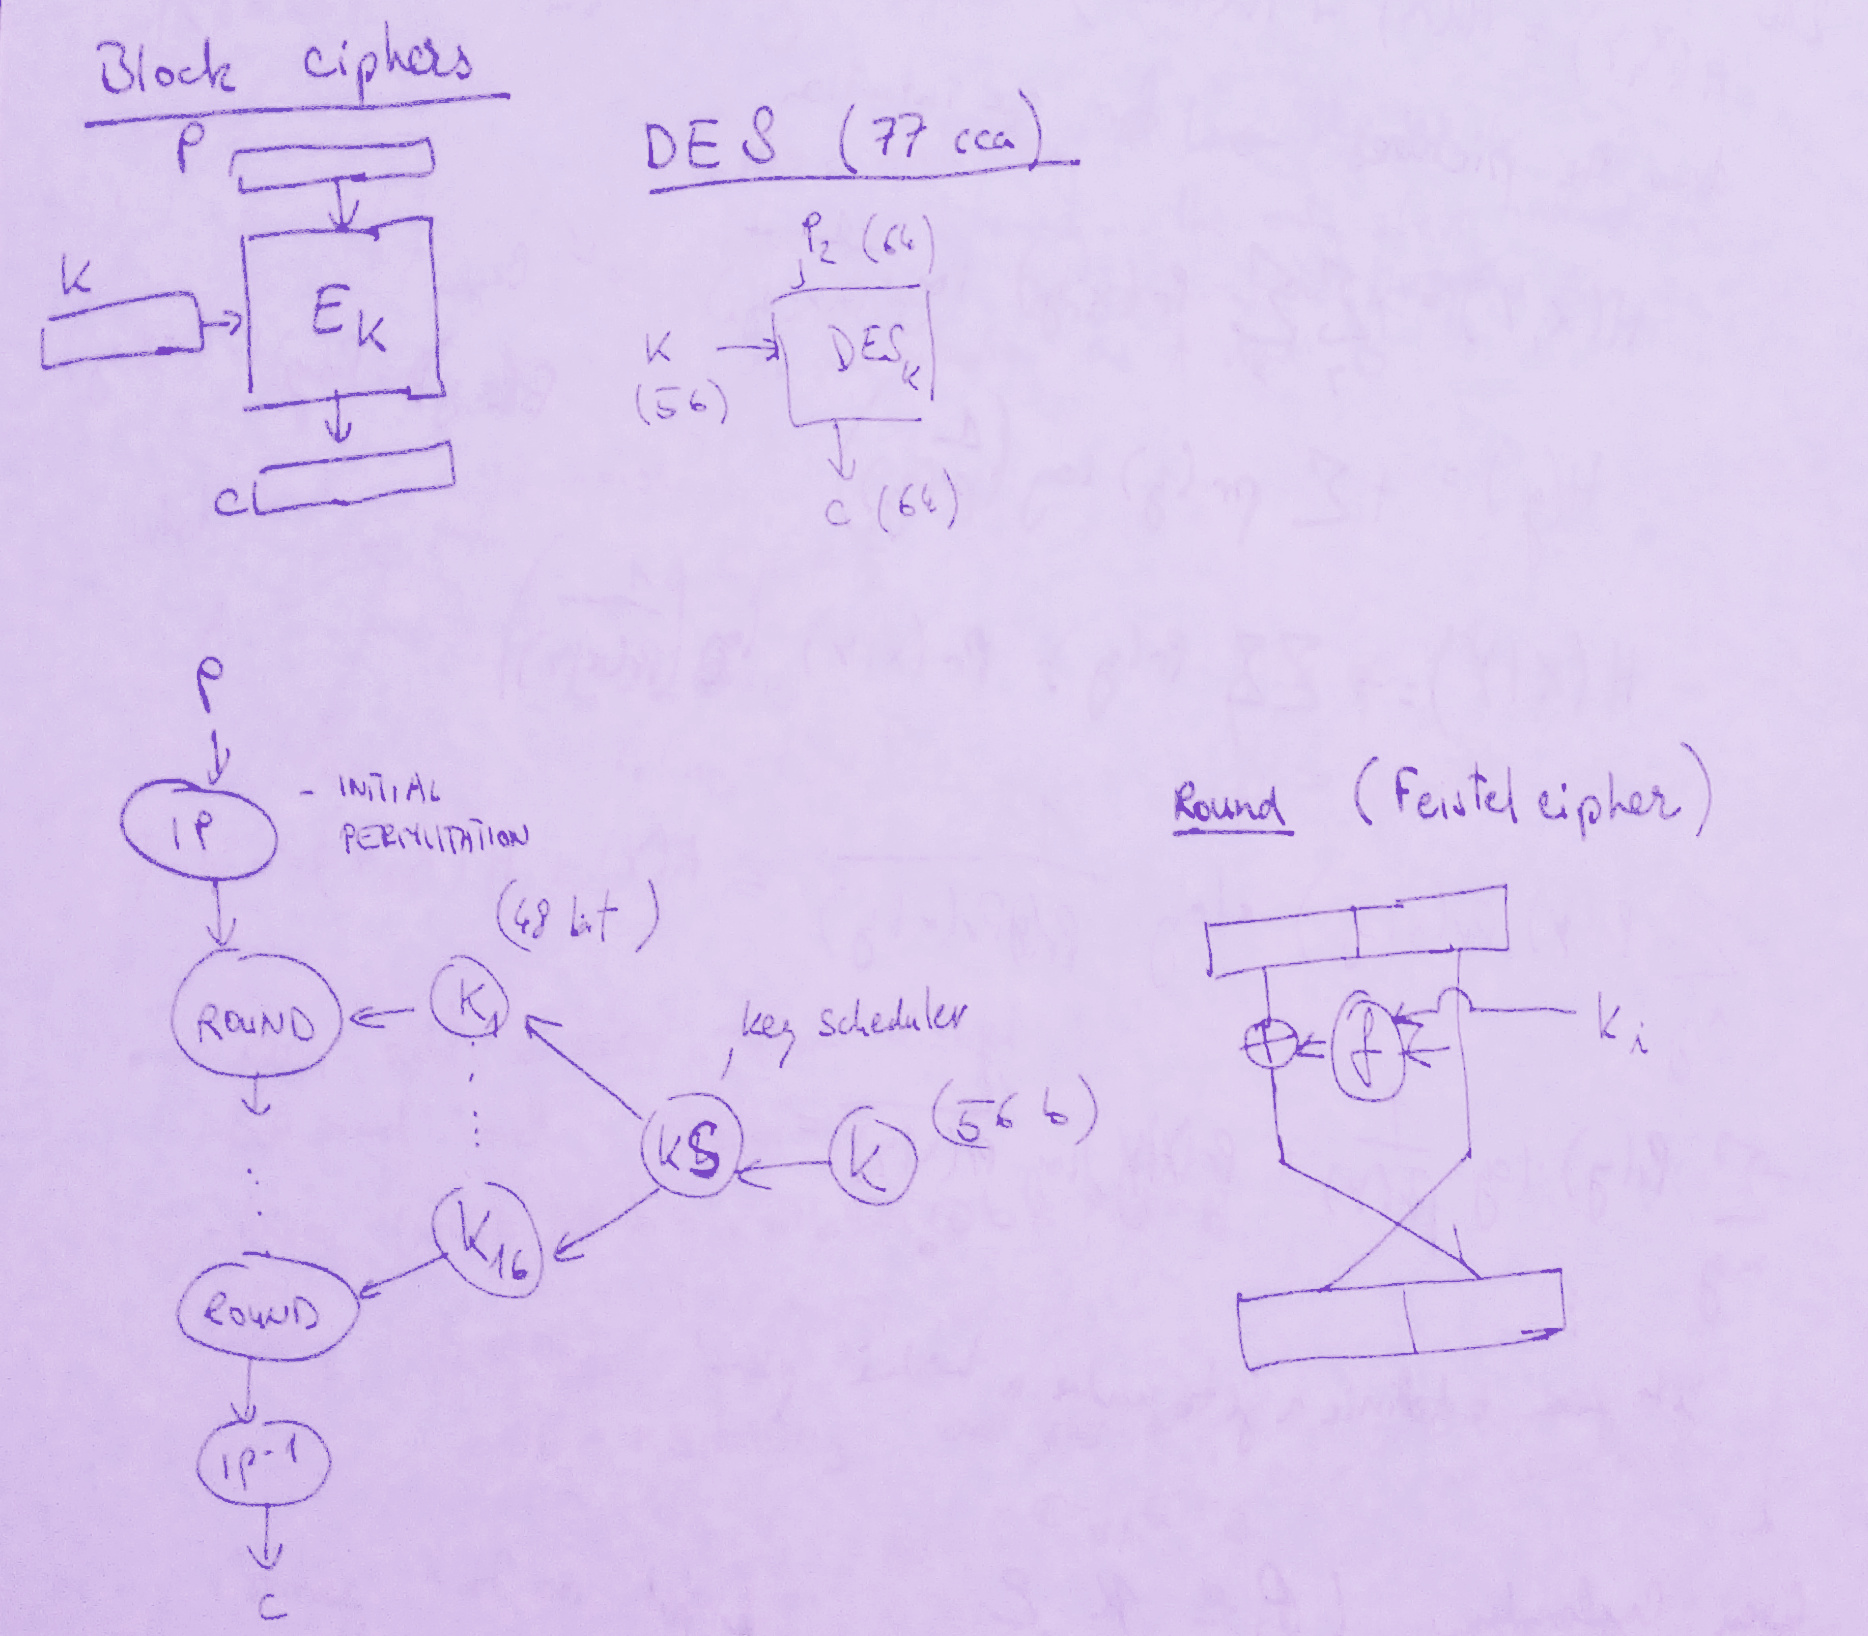
\includegraphics[width=0.5\textwidth]{DES.jpg}
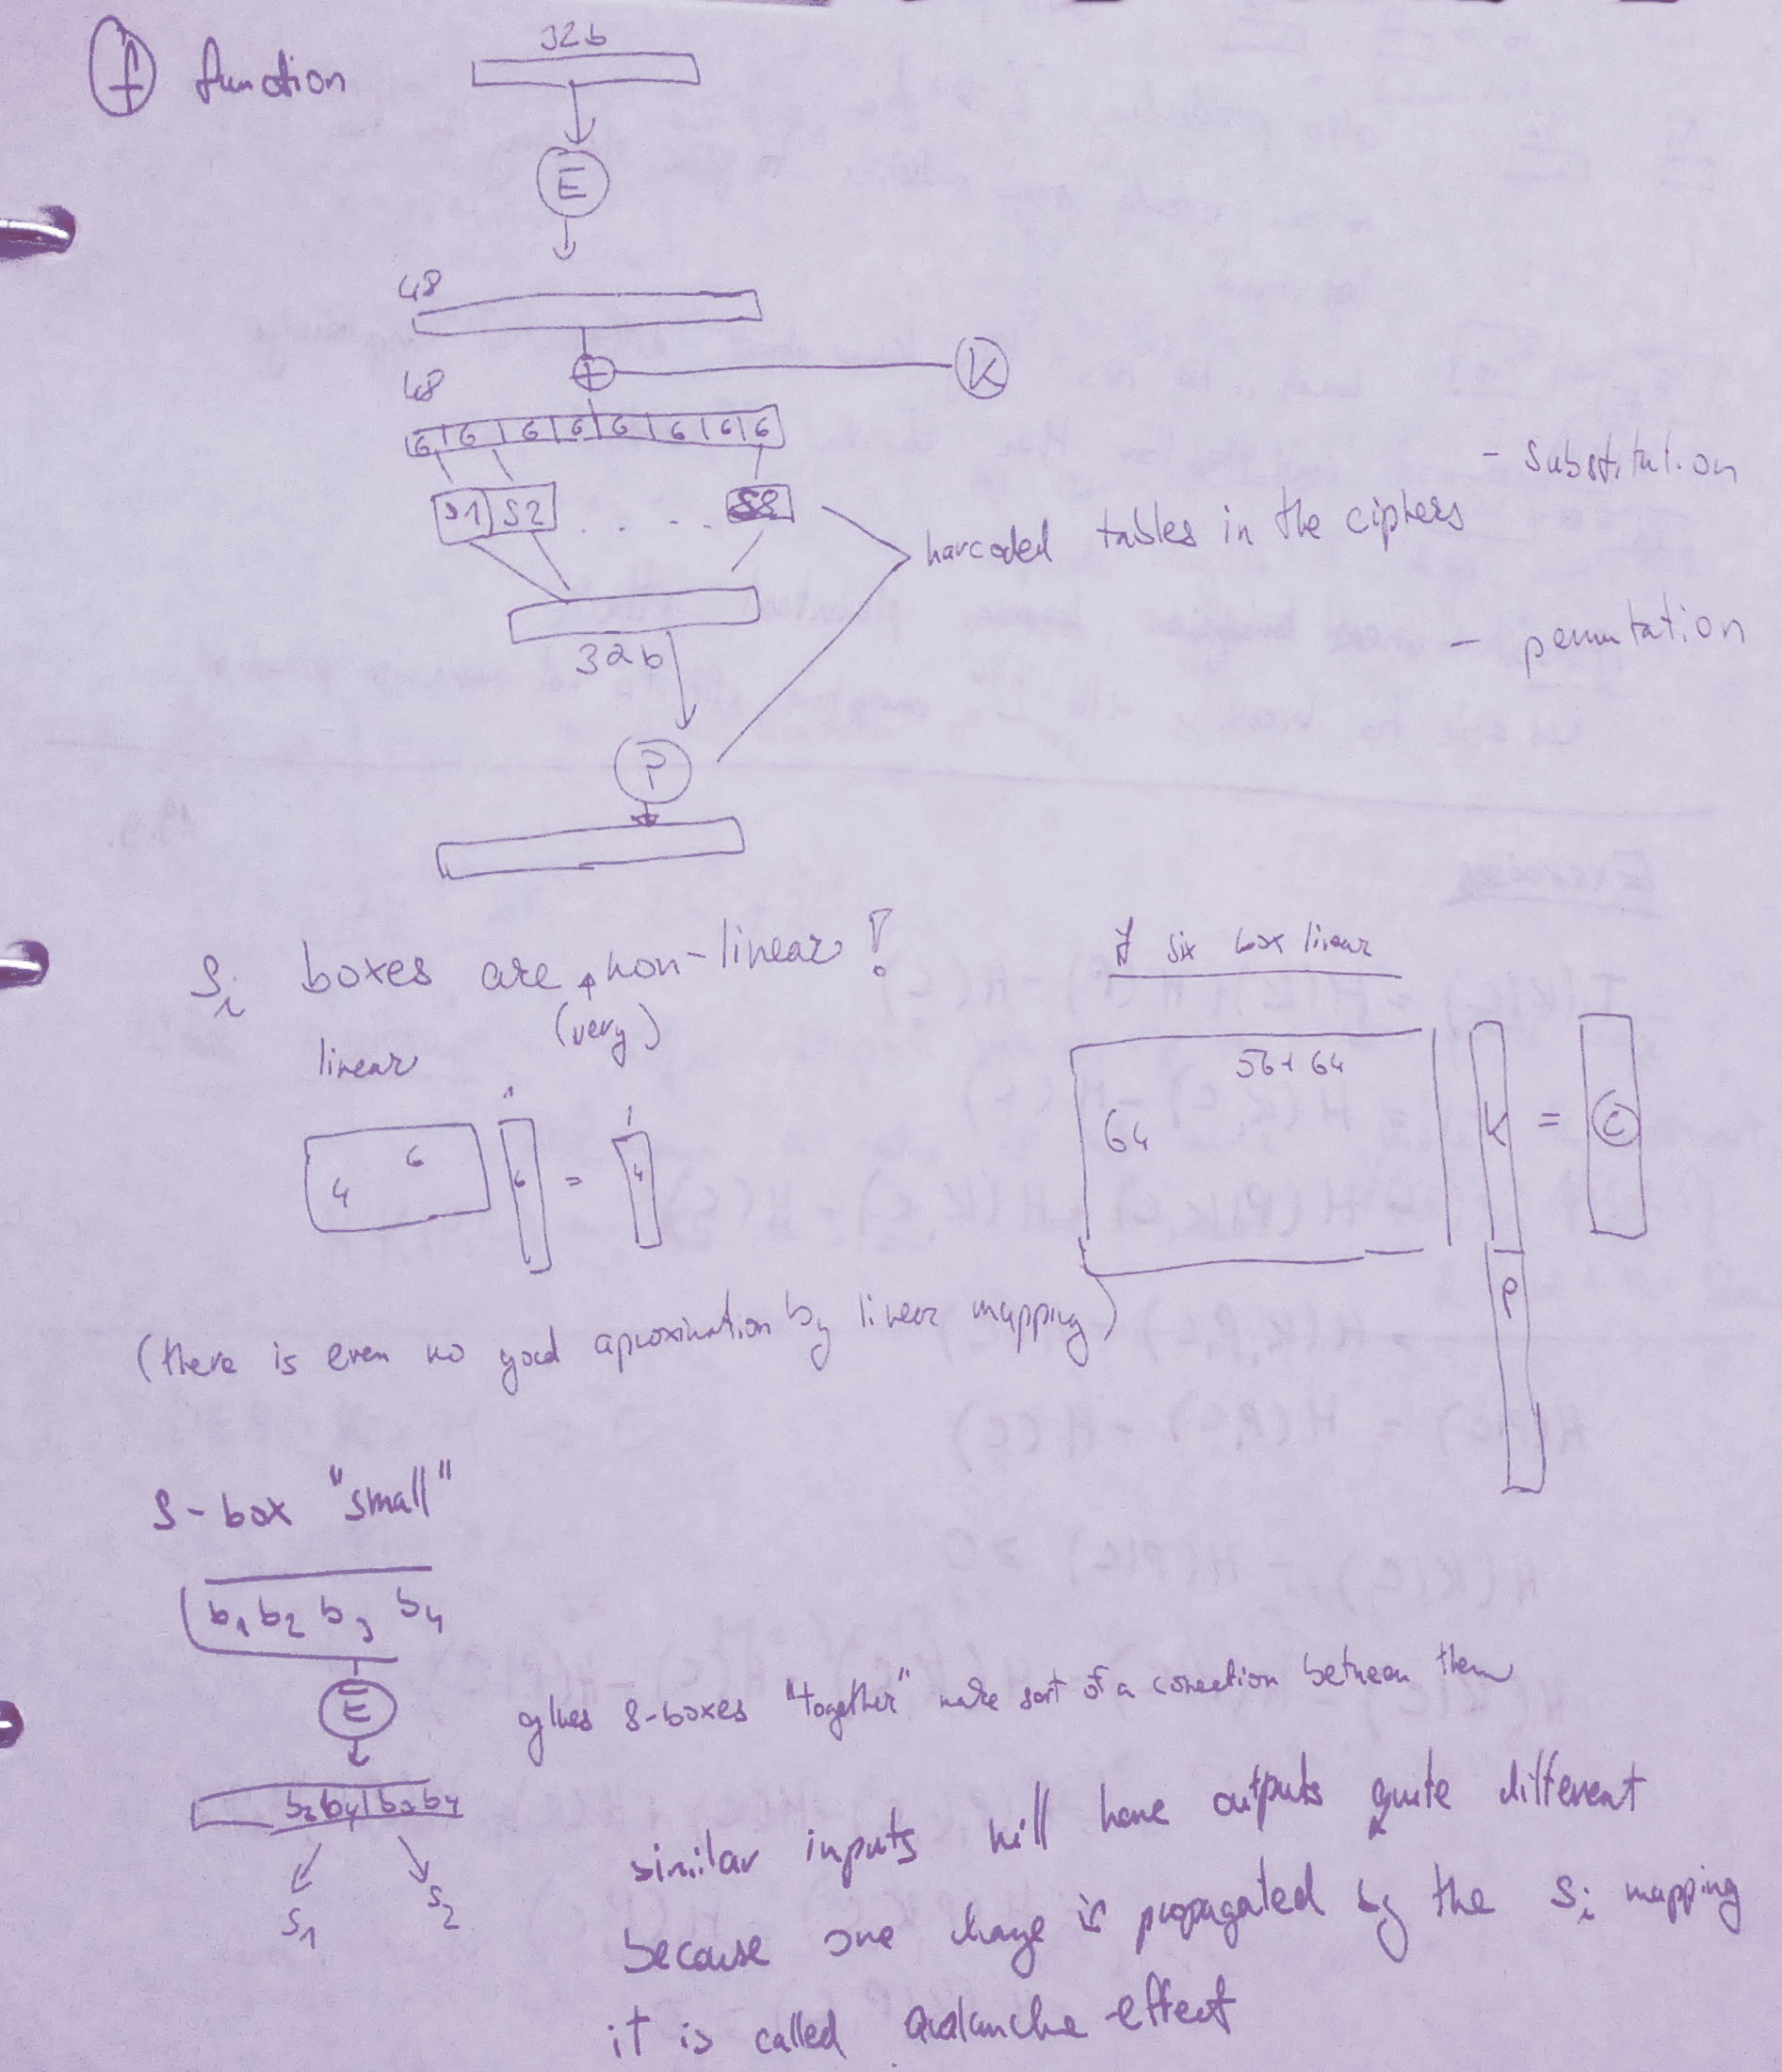
\includegraphics[width=0.5\textwidth]{des_F.jpg}
\begin{itemize}
\item Special version of iterrated feistel round (16 rounds, 64bit blocks, 56b key)
\item the reasons why it look like that are quick hardware and software implementation, in the last round the permutation is missing to be able to use the same HW just in reverse order to decode
\end{itemize}
\subsection*{AES}
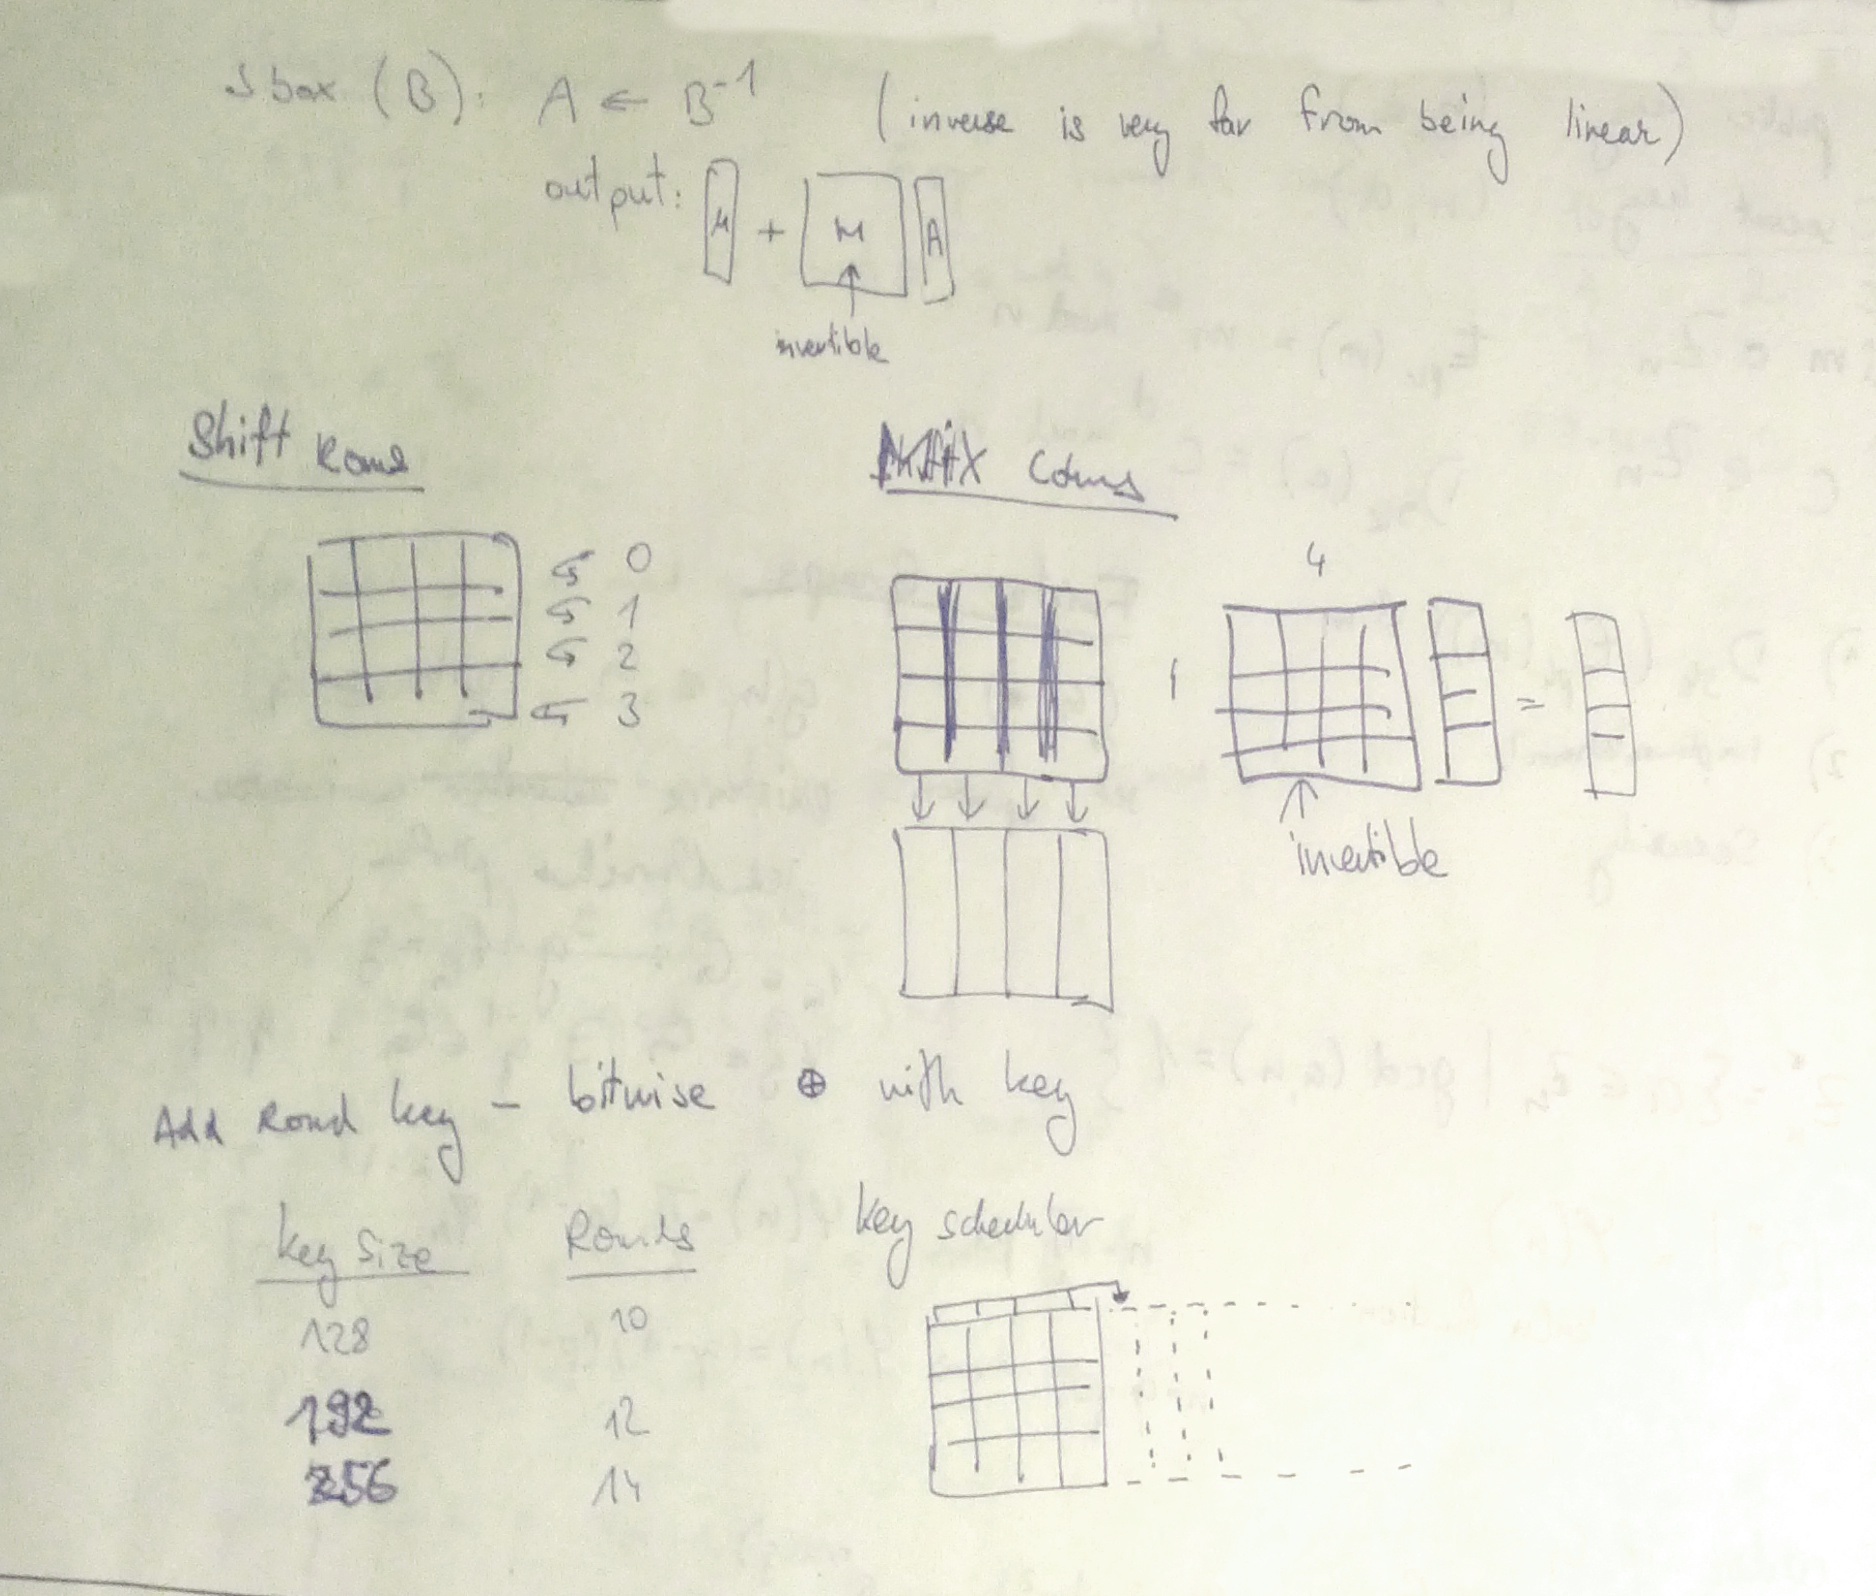
\includegraphics[width=0.75\textwidth]{AES.jpg}\\
The successor of DES, because the security even just for brute force attack was not enought (reminder - we can solve it with good probability in $2^\frac{k}{2}$ time (birthday paradox), basic implementation has 128k, 196b and 256b variants, again iterated 10, 12, 14 round respectively
High level description - should explain the picture
\begin{enumerate}
\item in the very beginning add $k_0$
\item number of rounds - 1 do
\begin{enumerate}
\item subbytes - method for substituting the letters, these operand are invertible - from two reasons - if they are, they are easy to invert and secondly the invertible operation is very far from being linear.
\item shift rows
\item mix columns
\item add round key with $\oplus$
\end{enumerate}
\item for last round omit mix columns -- similar reasons as for DES missing last permutation
\end{enumerate}
\subsection*{Linear cryptoanalysis}
\subsection*{Differential cryptoanalysis}
\subsection*{Security definitions}
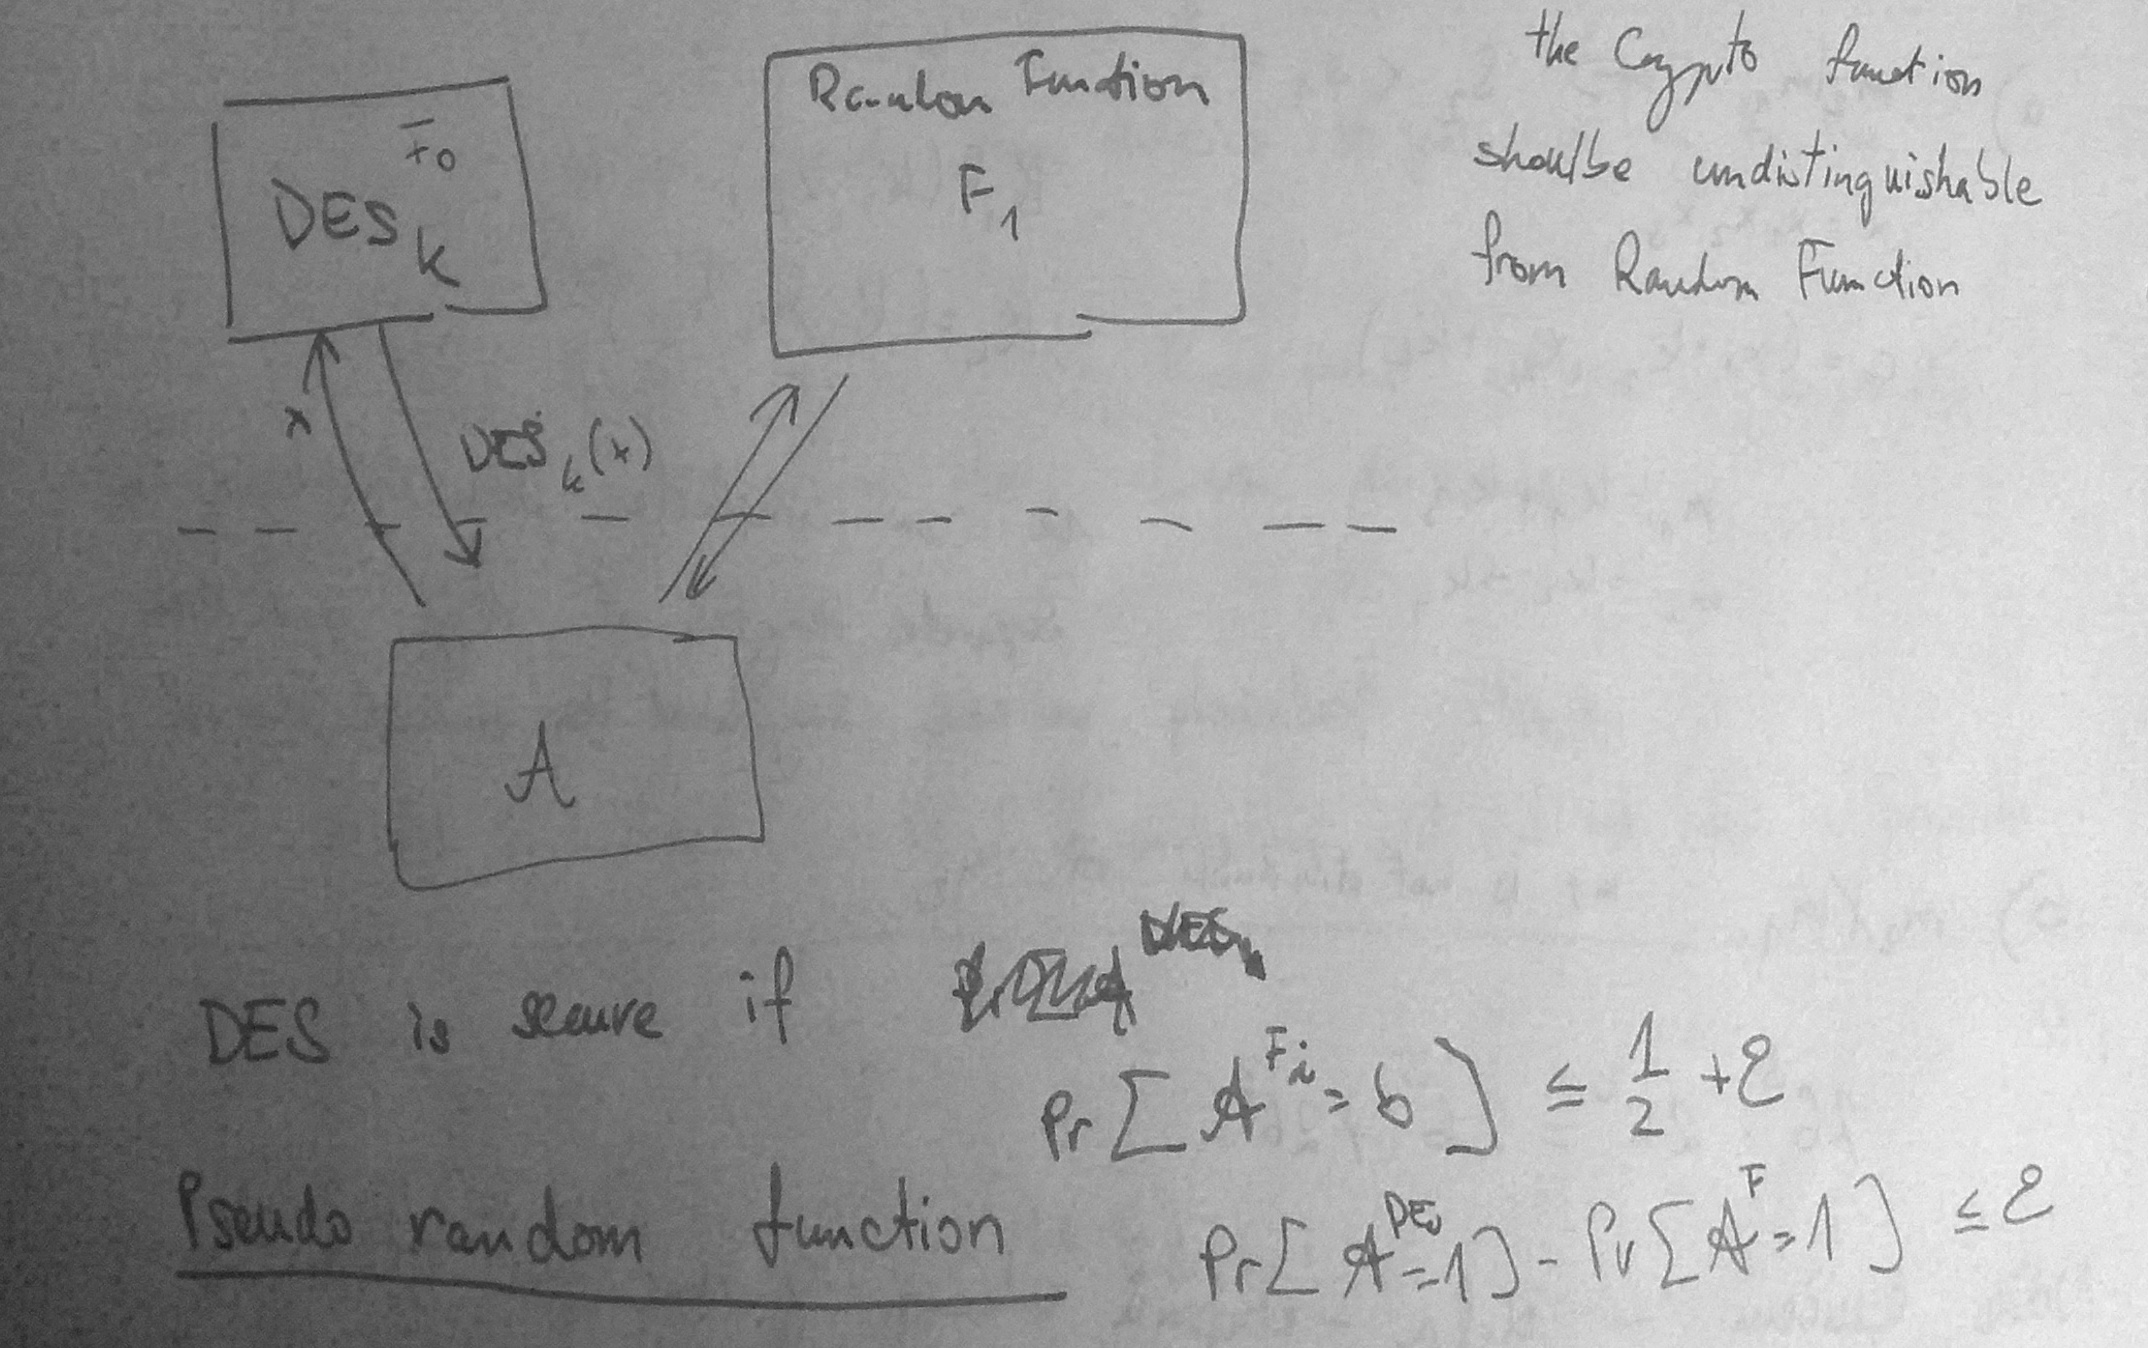
\includegraphics[width=0.5\textwidth]{PRF_security.jpg}
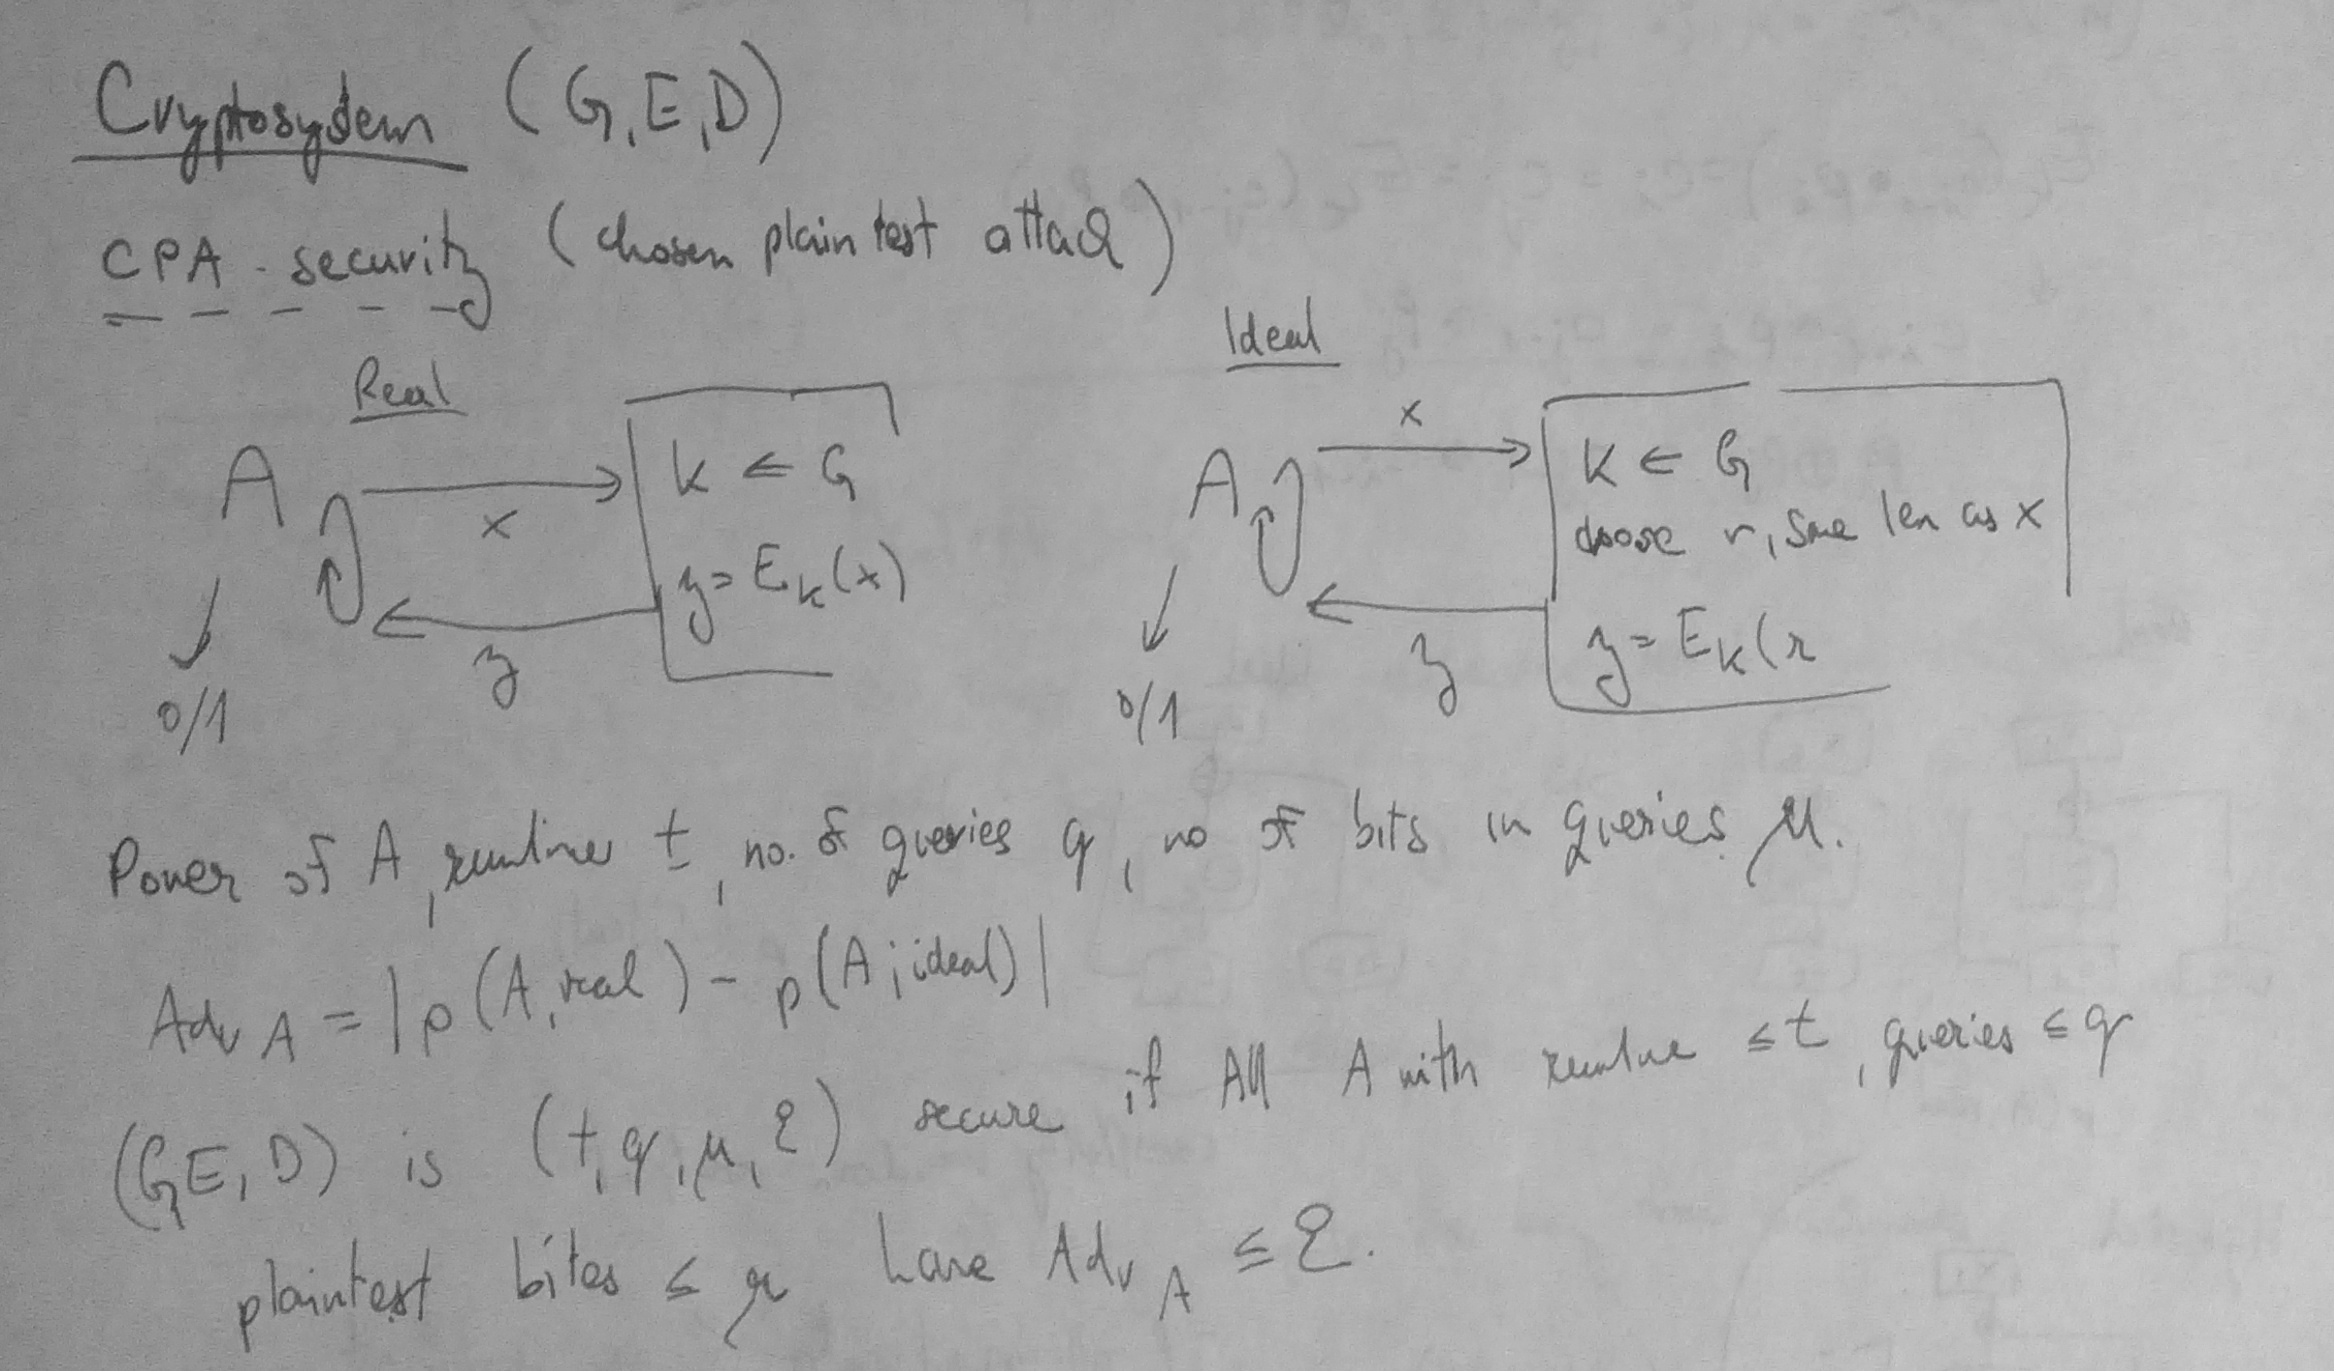
\includegraphics[width=0.5\textwidth]{CPA_security.jpg}
\subsection*{CBC and CTR}
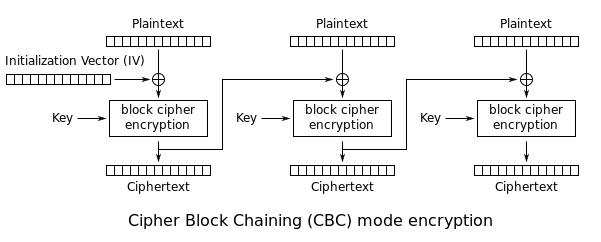
\includegraphics[width=0.5\textwidth]{CBC.png}
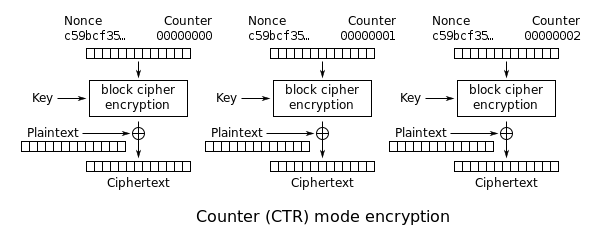
\includegraphics[width=0.5\textwidth]{CTR.png}

\end{document}